

%-----------------------------------------------------
\begin{frame}[allowframebreaks, fragile]{Named Entities}
\subsubsection{Named Entities, normalization and norm data}

\begin{block}{Persons vs. personal names}\small 
A \texttt{<person>} (person themselves) isn't identical with their \texttt{<persName>} (name = word = string of characters referring to a person)! 
\medskip

There are the following elements in the TEI: \texttt{<persName>} for \texttt{<person>}, \texttt{<orgName>} for \texttt{<org>} (organisation), \texttt{<placeName>} for \texttt{<place>}.\\

\texttt{<geogName>} (= geographical) = landscape markers (such as mountains, etc.) 
\end{block}

\framebreak

\begin{block}{Normalizing different names forms}\small
Problem: \textbf{Different name forms}, thus:
\bg{w3schools}{white}{Normalization:} Showing that \emph{one and the same} person is meant by giving out \textbf{identification (ID) numbers} on the internet and normalizing name forms. We can add that as a reference (\texttt{@ref}) to a list of persons in the TEI header, for example. 

We reference the information in this list using its \texttt{@xml:id} in \texttt{@ref} attribute in-text. \\

We can add norm data (such as GND, \emph{Gemeinsame Normdatei}, or \href{https://www.geonames.org/}{geonames}) using attributes, e.g. \texttt{@n} (\emph{label}) or \texttt{@ana} (interpretation). 
\end{block}

\green{\href{https://explore.gnd.network/search?term=michael\%20maier\&rows=25}{Try the GND explorer!}}

\framebreak

\bg{w3schools}{white}{Redundancy is a source of errors!} $\to$ reference one place where you can easily check if information is correct or update in just one place in case of changes -- store the information exactly once, if possible. 

$\to$ Mistakes happen and this way, you will only need to fix them once in one place, not 200 occurences. 
For unique references, use  \\
\verb|<person xml:id="Mina">Mina</person>|.

\begin{block}{\texttt{xml:id}}\footnotesize
  You can only have the same value for the \texttt{@xml:id} once in your document!  \\
You reference it using the \texttt{@ref} attribute prefaced by a hashtag (shorthand for `in this document' in the TEI): \\
\verb|<persName ref="#Mina">Mina</persName>|.
\end{block}

\end{frame}

%------------------------------------------------------------------------------
\begin{frame}[allowframebreaks,fragile]{\texttt{<tei:name>}}
The TEI offers a whole set of elements to denote names such as:


  \begin{columns}[T,onlytextwidth]
    \column{0.5\textwidth}
\begin{itemize}
    \item persName
    \item surname
    \item firstname
    \item name
\end{itemize}

\column{0.5\textwidth}
You could also simply use \texttt{<name>} and \texttt{@type} attribute to define which type of name it is. 
\begin{xmlcode}
<name type=„person“>
<name type=„pet“>
<name type=„vulgo“>
<name type=„house“>
<rs type=„name“>
\end{xmlcode}
\end{columns}

\texttt{<tei:name>} = 
\begin{itemize}
    \item concrete version of \texttt{<tei:rs>} (refering string)
    \item generalisation of \texttt{<persName>} (personal name)
\end{itemize}

\framebreak

  \begin{columns}[T,onlytextwidth]
    \column{0.5\textwidth}
      \begin{itemize}
    \item surname 
    \item forename 
    \item roleName (social role, e.g. King of France)
    \item addName (additional name) 
    \item nameLink (name link)
    \item genName (generational name component, e.g. sen., jun.)
    \item orgName (organization name)
    \item placeName
    \item geogName (geographical name)
\end{itemize}

    \column{0.5\textwidth}

     ``Eberhard, count of Württemberg''
\begin{xmlcode}
<persName>
  <foreName>Eberhard</foreName>
  <roleName>count of
    <placeName>Württemberg</placeName>
  </roleName>
</persName>
\end{xmlcode}

``Count Eberhard of Württemberg and his sons Ludwig and Ulric'' etc.


  \end{columns}
\end{frame}




%------------------------------------------------------------------------------
\begin{frame}[fragile]{Unique identifiers, noramlization, norm data\dots}

  \begin{columns}[T,onlytextwidth]
    \column{0.5\textwidth}
      \green{tei:placeName @key} points to the register of persons:
\begin{xmlcode}
<persName key="A000835">
  Heuschkel</persName>
\end{xmlcode}

which is the same as: \\
\protect\url{http://www.weber-gesamtausgabe.de/de/A000835}

or:
\begin{xmlcode}
<person xml:id="A000835">
\end{xmlcode}

    \column{0.5\textwidth}

      \metroset{block=fill}

      \begin{block}{modernisation?}\footnotesize
        Vienna = Wien, capital of Austria
      \end{block}

      \begin{alertblock}{main entry point?}\footnotesize
        Preßburg $\to$ Bratislava, capitol of Slovakia \\
also: Preßburg, Pozsony, Prešporok
      \end{alertblock}

      \begin{exampleblock}{identifier?}\scriptsize
        Bernardus Papiensis $\to$ VIAF-ID: 15126540 $\to$\protect\url{<http://viaf.org/viaf/15126540/>}

\textbf{main entry point:} Bernhard von Pavia, before 1150-18.9.1213
also: Bernardus Papiensis, Bernardo Balbi, Bernardus Balbus, Bernard of Pavie, Bernardus Circa, Bernardus praepositus Faventinus, Bischof Bernhard von Faenza, Bischof Bernhard von Pavia \dots
      \end{exampleblock}

  \end{columns}
\end{frame}


%------------------------------------------------------------------------------
\begin{frame}[allowframebreaks]{Norm data}
  The Virtual International Authority File (VIAF) is an international authority file.

  \begin{columns}[T,onlytextwidth]
    \column{0.5\textwidth}
      \begin{block}{Identifiers}
        Describe historical individuals (or places etc.) with a unique identifier using authority files or other norm data. 
Datasets linking information in that way are called \emph{Linked Open Data}, for example: Wikipedia pages list authority control information, collect information as Linked Open Data (Wikidata)
      \end{block}

    \column{0.5\textwidth}

      \metroset{block=fill}

      \begin{block}{Example 1}
        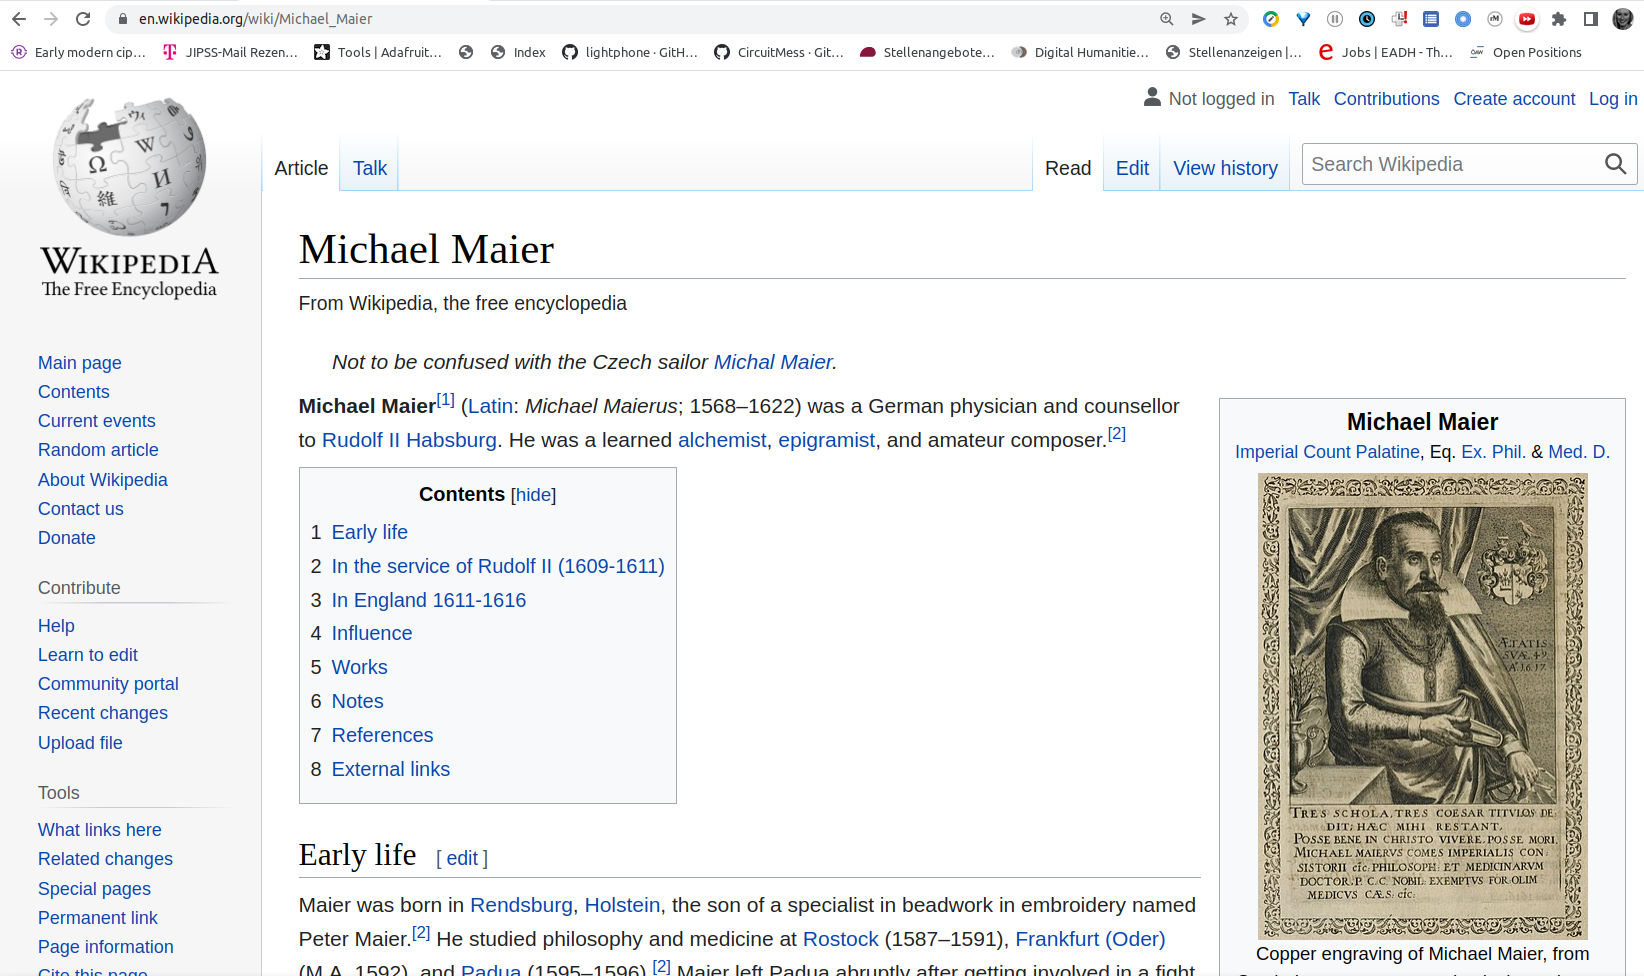
\includegraphics[width=0.95\textwidth]{img/mmaier-wiki1.png}
      \end{block}
      
            \begin{block}{Example 2}
        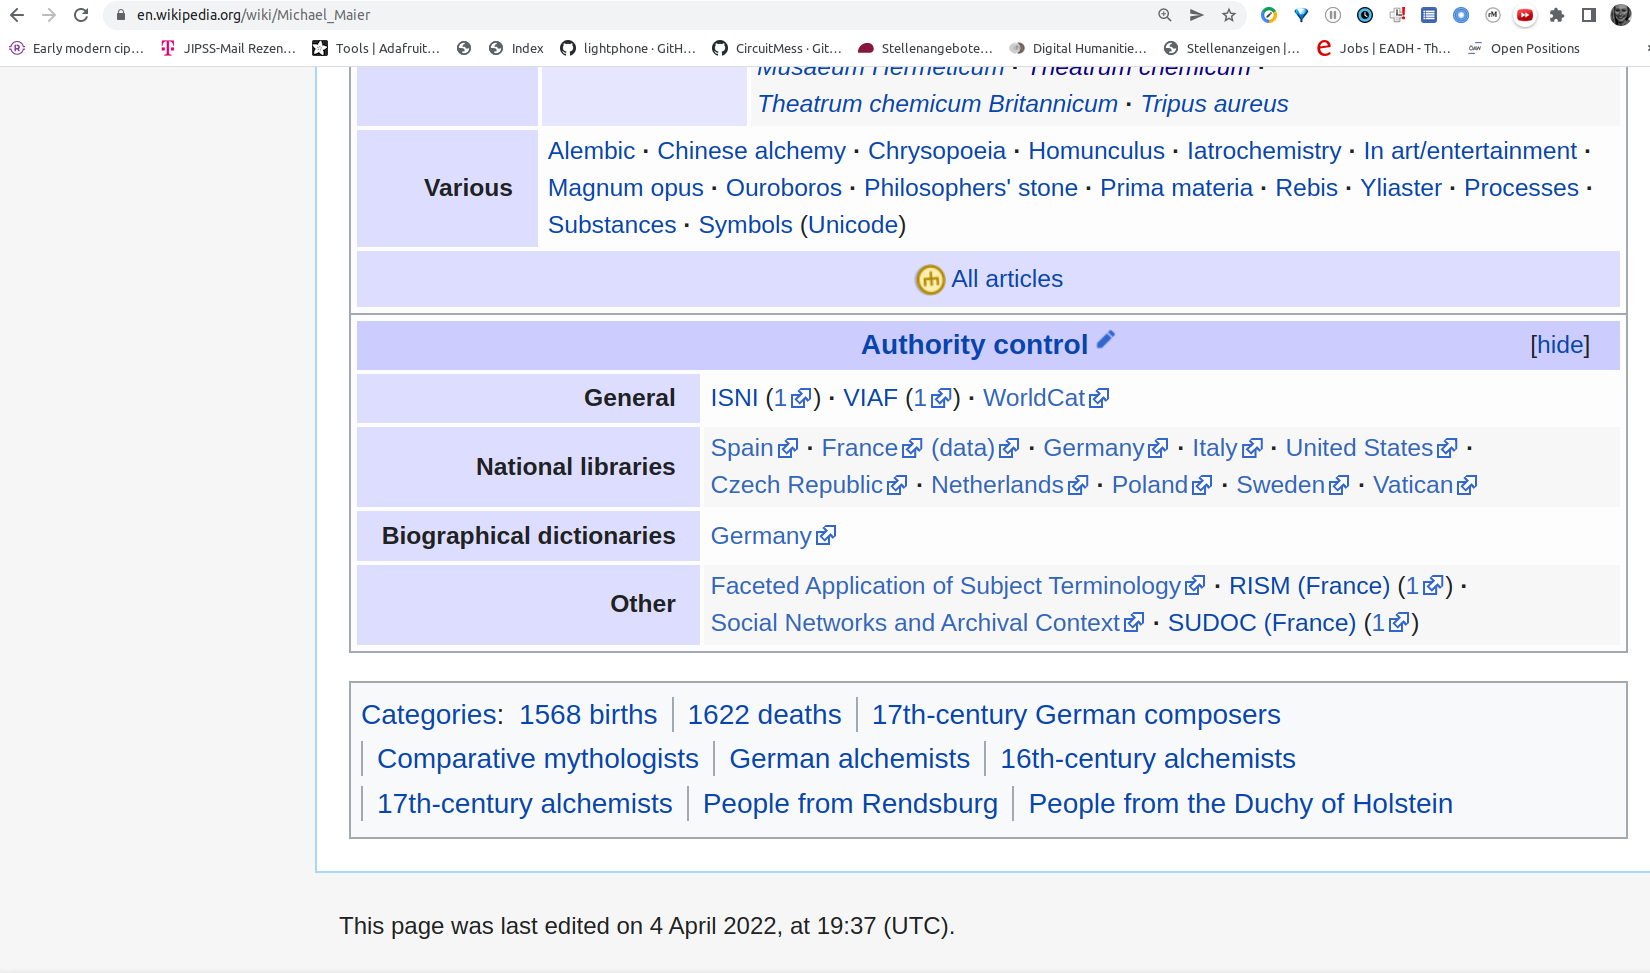
\includegraphics[width=0.95\textwidth]{img/mmaier-wiki2.png}
      \end{block}


  \end{columns}
  \framebreak
  
    \begin{columns}[T,onlytextwidth]
    \column{0.5\textwidth}
        \begin{alertblock}{Authority control}
        \begin{quote}
    In library science, \textbf{authority control} is a process that organizes bibliographic information, for example in library catalogs by using a single, distinct spelling of a name (heading) or a numeric identifier for each topic. (\href{https://en.wikipedia.org/wiki/Authority_control}{Wikipedia})
\end{quote}
      \end{alertblock}

      \begin{exampleblock}{Examples for norm data}\footnotesize
\begin{itemize}
    \item German \textbf{GND} (Gemeinsame Normdatei)
    \item \textbf{LCCN} (Library of Congress Control Number)
    \item \textbf{VIAF} (Virtual International Authority File)
\end{itemize}
      \end{exampleblock}
      
       \column{0.5\textwidth}
             
            \begin{block}{Example 3}
        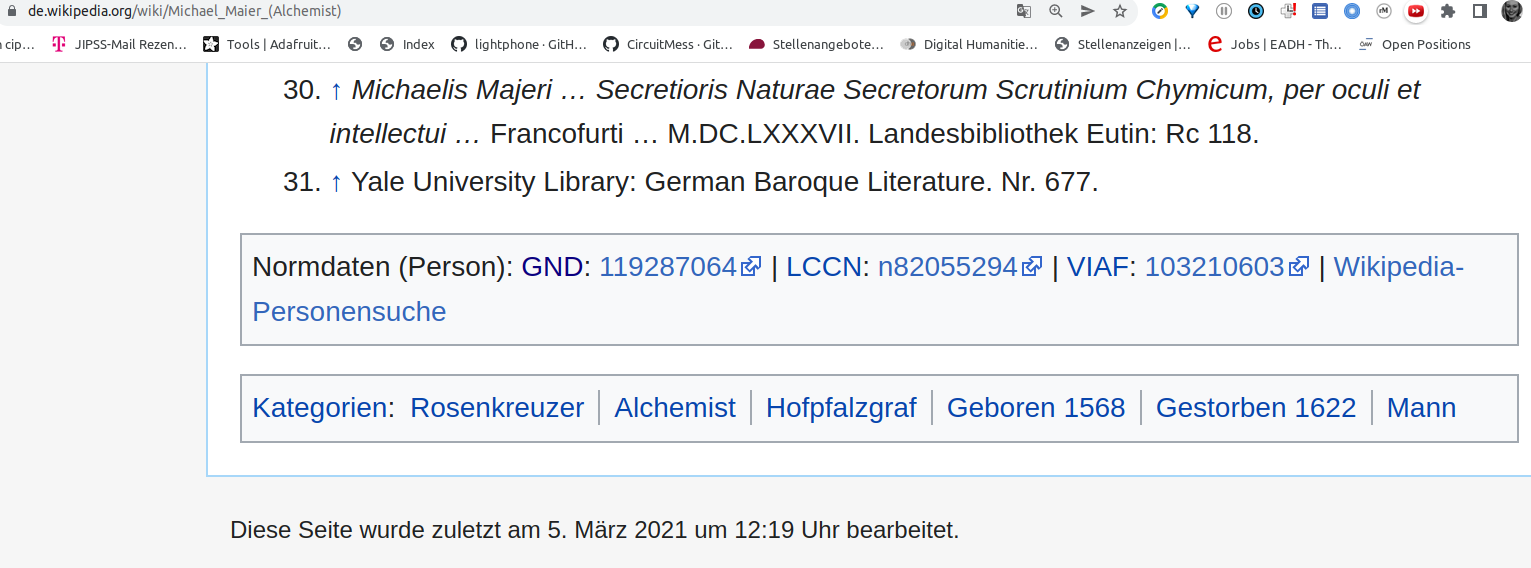
\includegraphics[width=0.95\textwidth]{img/mmaier-wiki3.png}
      \end{block}

      \end{columns}
\end{frame}




%-----------------------------------------------------
\begin{frame}[allowframebreaks]{Reminder: Making the TEI your own}
\small
\metroset{block=fill}

\begin{columns}
\column{0.5\textwidth}
    \begin{block}{How to find information on TEI elements}
    \dots and teach yourself how to use new elements:
\begin{itemize}\footnotesize
    \item General TEI guidelines (\href{https://tei-c.org/release/doc/tei-p5-doc/en/html/SG.html}{XML Primer}, \href{https://tei-c.org/support/learn/}{Learn the TEI page}, etc.)
    \item web-search TEI + (element you want to know about), i.e. ``tei teiHeader'' and you will get:
    \begin{enumerate}\scriptsize
        \item \href{https://www.tei-c.org/release/doc/tei-p5-doc/en/html/ref-teiHeader.html}{definition page}
        \item \href{https://www.tei-c.org/release/doc/tei-p5-doc/en/html/examples-teiHeader.html}{list of all examples for that element} $\to$ directly over websearch or click `show all' in the examples on the `definitons page'
        \item sometimes even an \href{https://www.tei-c.org/release/doc/tei-p5-doc/en/html/HD.html}{module overview text for things as big as \texttt{<teiHeader>}} (has its own module)
    \end{enumerate}
\end{itemize}
    \end{block}


\column{0.45\textwidth}

\begin{block}{Module 13:}
\href{https://tei-c.org/release/doc/tei-p5-doc/en/html/ND.html}{Names, Dates, People, and Places}.
\end{block}

\begin{block}{}
\footnotesize
Also: The TEI guidelines are documentation and reference, not necessarily ideal teaching tools $\to$ overwhelming. 
Maybe try other tutorials like the \href{http://gams.uni-graz.at/o:dhoxss2016-tei-names}{these slides}.
\end{block}

\end{columns}

\end{frame}

